\documentclass{article}

%%%%%%%%%%%%%%%%%%%%%%%%%%%%%%%%%%%%%%%%%%%%%%%%%%%%%%%%%%%%%%%%%%%%%%%

\usepackage{url}
\usepackage{graphicx}
%\usepackage{fullpage}

% Remove red border around refs and make them stand out.
\usepackage[colorlinks=true,linkcolor=blue]{hyperref}

%%%%%%%%%%%%%%%%%%%%%%%%%%%%%%%%%%%%%%%%%%%%%%%%%%%%%%%%%%%%%%%%%%%%%%%
%% Check these macro values for appropriateness for your own document.

\title{IS3 Group Report}

%%authors
\author{
  Richard Fleming \\
  James Gallagher \\
  Craig McLaughlin \\
  Victor Pantazi \\
  Gordon Reid \\
  Ross Taylor}

%%release date 
\date{\today}

%%%%%%%%%%%%%%%%%%%%%%%%%%%%%%%%%%%%%%%%%%%%%%%%%%%%%%%%%%%%%%%%%%%%%%%

\begin{document}

%%%%%%%%%%%%%%%%%%%%%%%%%%%%%%%%%%%%%%%%%%%%%%%%%%%%%%%%%%%%%%%%%%%%%%%

\maketitle

%%%%%%%%%%%%%%%%%%%%%%%%%%%%%%%%%%%%%%%%%%%%%%%%%%%%%%%%%%%%%%%%%%%%%%%
%% Standard section for all documents

\section{Preamble}

In this report, various popular calendars are evaluated using the
Think-aloud evaluation technique to identify desirable features of a
modern calendar. Three paper prototypes are designed by pairs from the
team, and based on these paper prototypes, a final paper prototype will
be detailed.

%%%%%%%%%%%%%%%%%%%%%%%%%%%%%%%%%%%%%%%%%%%%%%%%%%%%%%%%%%%%%%%%%%%%%%

\section{Overview}

The prototypes were based on the Facebook, OS X, Evolution on Scientific
Linux, 30 Boxes, and Google calendars. For prototyping and evaluating,
the team split up into two person sub-teams. For the purposes of the
discussion the teams are labelled based on the calendars they evaluated.

The final paper prototype was a combination of the findings from the
calendars.

%%%%%%%%%%%%%%%%%%%%%%%%%%%%%%%%%%%%%%%%%%%%%%%%%%%%%%%%%%%%%%%%%%%%%%

\section{Calendar on OS X}

Apple Inc.'s use of skeuomorphism creates an interface similar to a real 
calendar with simulated page rips, faux-leather textures for UI
elements, and page turn animations. The design of the paper prototype
based on this calendar borrowed from the ethos of Apple's design.

\subsection{Think-aloud Evaluation}
The participant was asked to perform a series of set tasks, incorporated
into a scenario. The participant noted feeling uncomfortable during the
evaluation as it was unnatural for the them to have to vocalise their
actions. At some points during the experiment, the participant seemed
confused or surprised by the feedback from the system, occasionally
expressing uncertainty on how to proceed further with the task.

Below the tasks are described and feedback from the participant noted:

\begin{itemize}
\item Add an event for a friends party.

There was an intuitive plus button on the top-left of the window, which
opened a dialog box for adding an event on the currently selected day.

\item Change the event to the following week.

The calendar has a very intuitive drag and drop feature to move an
event from one day of the month to another. However, this feature does
not work across months; trying to move it to the next month cancels
the drag and drop operation.

\item Set a recurring event.

The participant noted that there was a nice repeat option which has
a number of common recurrence patterns, e.g. weekly, monthly, etc, and
an option for selecting the end date of the repetition.

\item Find out which days of the month are the busiest and quietest
respectively

The year view for the calendar fills days in colour indicating the
number of appointments scheduled for that day, in a spectrum from
red (busy) to white (quiet). This made this particular task incredibly
simple and it is this reason this feature was included in an early
paper prototype (see Section~\ref{sec:osxpp}).

\item Change the calendar categories currently displayed.

Calendar categories are displayed on a pane on the left side of the
screen with tick boxes indicating which categories are currently being
shown in the main view. To change which categories are displayed, it is
a simple matter of ticking the boxes of the desired categories.

\end{itemize}

\subsection{Paper prototype}
\label{sec:osxpp}

The paper prototype has a minimalist design with three views: week,
month, and year. These views are available through three buttons that
are always on the screen at the top centre-right. The currently selected
view is coloured differently than the others and appears depressed.

The initial draft of the event dialog pop up window, that would be
shown when a user decides to add a new event, or wishes to edit or
delete an existing event, is illustrated in Figure~\ref{fig:addevent}.

A user is able to have multiple calendars, perhaps to split up work and
home events. The screen (Figure~\ref{fig:viewcal}) allows a user to
choose which calendars to view, add a new calendar, or delete an old
calendar and associated events.

The month view for the calendar is shown in Figure~\ref{fig:monthview}.
This view is also the default view. Events are listed in summary form
in the grid of squares. When a user clicks on the grid, the full listing
for the selected day is shown in the side panel on the right.

The year view for the calendar is depicted in Figure~\ref{fig:yearview}.
The primary purpose of this view is to allow daily summaries to be
visualised. Similar to Apple's Calendar application, days which are
busy are coloured in an increasing level of opaqueness, dependent on
the number of events added for the associated day.

\subsection{Think-aloud Evaluation of paper prototype}

To evaluate the paper prototype that was designed, one member of the
design team for this prototype acted as the evaluator, and a member
from a different sub-team acted as the user. The same tasks as before
were used to evaluate the system. The participant noted that the
prototype had a minimalist and aesthetic design. It was easy to see the
system status because the currently selected view is displayed as a
selected button next to the other view options. The participant was not
sure how to enter dates for event information, whether they had to
provide the correct format (including /'s) or not.

%%%%%%%%%%%%%%%%%%%%%%%%%%%%%%%%%%%%%%%%%%%%%%%%%%%%%%%%%%%%%%%%%%%%%%

\section{Evolution on Scientific Linux}

This paper prototype was designed using the findings from the evaluation 
of Evolution on Scientific Linux. Overall, the evaluation showed
dislike for most of the features of Evolution and as such most of the
features of this prototype are improvements on features of Evolution.

\subsection{Paper Prototype}

The first thing that was noticed about Evolution was that there was not
always a clear indication of the current system state. So for the
prototype a clear `Day/Week/Month/Year' section was included at the
top of the screen which also allowed the user to quickly switch between
views. The only paper prototype created was for the Month view due
to time constraints but the other views would have conformed to the
same general layout (i.e the sidebar and the ability to switch views
should be present in all views).

Another indicator of system state added was a check box section on
the left of the main view to allow users to select different categories
of event to be displayed, possibly having multiple categories shown at
any one time. Also, related to event categories, Evolution's
system for adding a new category was rather unintuitive so a
clear indication in the categories section of the sidebar labelled
`Add New' was added to this paper prototype.

Inconsistencies were found whilst using the Evolution system which
prompted the decision to have different views in this prototype to
have the same features available (i.e. the sidebar feature and the view
indicator).

The user should also be able to double-click on an event in any view and
have a summary of that event displayed in the lower section of the
sidebar. This decision was made because Evolution took the user to a
seperate page to view a summary which seems unnecessary.

All of the adding, editing and deleting events on this prototype was 
handled from the menu bar at the top of the screen. For the final
prototype it was decided that this was not a particularly practical
solution and that this functionality would be better handled from the
main view.

\subsection{Think-aloud Evaluation of paper prototype}

To evaluate this prototype, a member of the team not involved in this
particular design completed some tasks using this prototype.

Below are the findings from the evaluation:

\begin{itemize}
\item Add an appointment.

The user experienced some difficulty whilst adding an appointment,
although they did successfully complete the task, the process took a
little longer than expected. The user voiced his distress that he was
unable to simply click on a day and have the option to add pop up.
Instead in prototype design all core actions are kept inside the
File menu, believed to be intuitive, however the user felt that
the design lacked a connection between system-orientated design and
real world use, and commented on the lack of visibility for such a
simple feature.

\item Deleting an appointment.

This simple task also gave the user problems. The user's eye was
automatically drawn to the event summary and spent time looking for a
delete button before being told by the designer to look elsewhere.
The participant was unable to perform task without the aid of the
designer, who informed them they had to right click the selected event
day box in order for the option to delete to appear. Basic event
inconsistency was apparent here as the user had to go to the file menu
bar to add an event, but could right click the event to delete, both
should be possible through similar methods as they are related actions.
Also, the action was not clearly visible to the user, indicating a
problem with the design.

\item Change views from month, to week, to day.

The participant was able to complete the task quickly and simply with
clear access to the commands at the top of the screen. The user
commented on the clear visibility of the options, and pleasant
minimalist design.

\item Set a recurring appointment.

The user was able to navigate to the correct place to add a recurring
appointment as they realised it was most likely just an extension to
adding an appointment. Whilst in add appointment they successfully
clicked the recurring button which took them to a new screen where they
could set the details of the recurring appointment. However, the user
expressed that setting a start date then the number of occurrences of
the event was not the most user friendly method as it required them to
do some mental math to figure out when the event will end. A solution
they advised was to include an input box for end date as this meant 
the user would not need to calculate and do any extra work themselves.

\item Find out which days of the month are the busiest and quietest
respectively

In the prototype, a mini calender on the left hand side is visible
regardless of which view you are currently in. In this mini calender
each of the days has a colour indicator showing how busy that
particular day is; white meaning not busy, orange being moderately
busy and red meaning very busy. The user understood this when looking
at the prototype without any explanation and delared that this feature
was very intuitive even for a novice user and complimented the design
saying it was simple and minimal.

\item Set different categories for university, social and job
appointments.

Once the user was able to figure out how to add appointments, setting
different categories was a very simple extension. Simple tick boxes
made the task simple and quick to complete.

\item Change the calendar categories currently displayed.

Again the user was very impressed with the design choice to have a
small category section on the middle left of the UI. The user was able
to complete the task quickly and simply with clear access to simple
tick boxes for category selection. 

\end{itemize}

%%%%%%%%%%%%%%%%%%%%%%%%%%%%%%%%%%%%%%%%%%%%%%%%%%%%%%%%%%%%%%%%%%%%%%%

\section{Google, Facebook, and 30 Boxes calendars}

\subsection{Google calendar}

Most of the team is familiar with the Google calendar design, and as
such, it has influenced the prototype greatly. The day view on the
right is inspired by this calendar.

%%%%%%%%%%%%%%%%%%%%%%%%%%%%%%%%%%%%%%%%%%%%%%%%%%%%%%%%%%%%%%%%%%%%%%

\subsection{Facebook Events calendar}

Facebook's Events calendar is shaped by the company's focus on social
interaction. As such, events are geared towards social activities, and
leave a lot to be desired for a private, personal calendar. The
evaluation showed that this calendar only has two features that
might be useful : the ability to share easily with your friends,
and the integrated Bing Maps for appointment location, which could be
used to calculate if the user has time to travel between two
appointments at different locations.

%%%%%%%%%%%%%%%%%%%%%%%%%%%%%%%%%%%%%%%%%%%%%%%%%%%%%%%%%%%%%%%%%%%%%%%

\subsection{30 Boxes online calendar}

The 30 Boxes online calendar presents the user with a minimalistic yet
informative view of the following fortnight's events and the previous
week's activities. The design of one sub-team's paper prototype was
influenced by this calendar. 

\subsection{Think-aloud Evaluation}

One of the sub-team members played the role of a regular user and was
asked to complete a series of tasks, while the other team member noted
down any feedback provided:

\begin{itemize}
\item Create an appointment on a given day

Although there was no visual indication of how to add an event to a
specific date, the user guessed correctly that a simple click on that
day would work.

\item Move that appointment to a different day

The user edited the appointment's date manually, without realizing that
he could drag and drop.

\item Set a recurring appointment with a given duration

30 Boxes has a nice feature that lets you specify recurrences that
do not have a pattern.

\item Find the busiest and quietest days of the month

There is no easy way to see the busiest days because of box size
limitation.

\item View just one category of appointments

If a user has many different categories, deselecting them one by one is
tedious.

\item Other comments :

Using a context-aware interface (e.g. clicking in front of a week row
switches to that week's view) may not be intuitive to novice users.

\end{itemize}

\subsection{Paper Prototype}

This sub-team then designed a paper prototype based on a merging of the
Google calendar day view and the 30 Boxes month view. The idea of this
prototype is to convey as much relevant information as possible on a
single view. A user can click on any day and the day view on the right
will update with those day's appointments, ordered by time. Other
features are: colours can be used to represent different categories
of appointments, appointments can be moved to different days by
dragging and dropping them into different day boxes from the day
view on the right to the month view on the left, and there are now
explicit buttons for switching to a week or year view in the top
left corner. 

Another action focused on was the actual creation of a new
appointment. A user might be overwhelmed by calendars that provide many
fields that have to be completed to create a simple appointment.
The appointment creation pop-up, designed in this prototype, is split
into pages, and a valid appointment only needs the information on the
first page to be created that is, just a name and time. The other
fields are available on the next page, accessible through a link in the
bottom right corner of the pop-up. There a user can specify repetition,
add reminders, add a location, assign a category, share with others or
add extra details about the appointment.

\subsection{Think-aloud evaluation of paper prototype}

The same tasks were used to evaluate the prototype as the 30 Boxes
Think-aloud evaluation, noticing there still were problems finding the
busiest days in the month and adding an appointment to a day in a
clear, unambiguous way for the user. As such, the final prototype has a
plus button for adding events, and uses colour to convey the days which
are busy.

%%%%%%%%%%%%%%%%%%%%%%%%%%%%%%%%%%%%%%%%%%%%%%%%%%%%%%%%%%%%%%%%%%%%%%

\section{The final prototype}

The team discussed the findings from the evaluation of the early
prototype designs and used them to design the final version of the
prototype.

The summary of events for the currently selected date was a popular
feature amongst the prototypes, as was having the different time
division buttons (e.g. week, month, year, etc) always visible at the
top of the screen.

The `Add event' operation can be performed in two different ways, via
the regular systems-orientated approach by using the menubar's Event
menu, or by hovering the pointer over the desired date which causes a
small pop-up with a plus icon to appear. Clicking on the plus button
will display an event dialog window with the start date set to the
date the user hovered over. Each event belongs to one calendar category
which can be changed via the`Set category' button in the dialog window.
The categories are represented as radio buttons and a name.

The aim of the design was to keep the user interface free from clutter
so, the categories view of calendars was not included as its own panel
in the main view; even though this increases system status, it was
decided to allocate more screen real estate to the main view and create
a menu item for viewing the categories. The categories currently on
display in the main view can be changed via the Category menu by
selecting the `View categories' option. A dialog window similar to
an event's category dialog, except the categories are represented as
checkboxes indicating the possibility of multiple selection, will
pop-up showing all categories, with a checked box next to those that
are currently displayed.

Inspired from the OS X-based, and Evolution-based paper prototypes, the
final design has colour-coded days for the year view which indicates
the number of activities in a particular day.

While the feature of 30 boxes to allow repetition of an event even
though there is no pattern in the dates was a unique, interesting
feature, the number of people that would use this feature was
considered, by the team, to be small and hence, the benefit gained
from including this in the final prototype did not outweigh its cost.

%%%%%%%%%%%%%%%%%%%%%%%%%%%%%%%%%%%%%%%%%%%%%%%%%%%%%%%%%%%%%%%%%%%%%%%

\section{The Video}

\url{http://www.youtube.com/watch?v=yAREKMqu538}

\pagebreak

%%%%%%%%%%%%%%%%%%%%%%%%%%%%%%%%%%%%%%%%%%%%%%%%%%%%%%%%%%%%%%%%%%%%%%%

\appendix

\section{Figures for Calendar on OS X}

\begin{figure}[hb]
\centering
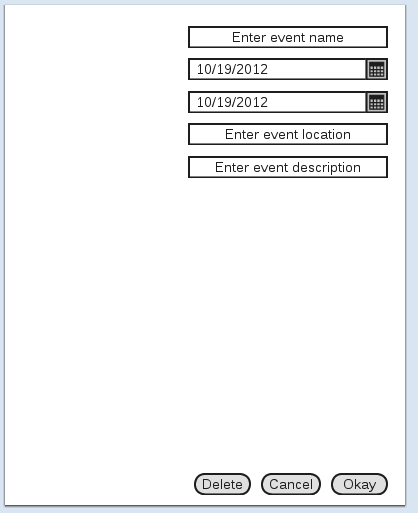
\includegraphics[scale=0.7]{CMCLGDREvent.png}
\caption{Add Event Dialog}
\label{fig:addevent}
\end{figure}

\begin{figure}[hb]
\centering
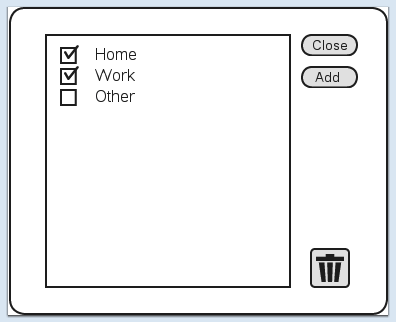
\includegraphics[scale=1]{CMCLGDRViewCalendar.png}
\caption{View Calendar Dialog}
\label{fig:viewcal}
\end{figure}

\begin{figure}[hb]
\centering
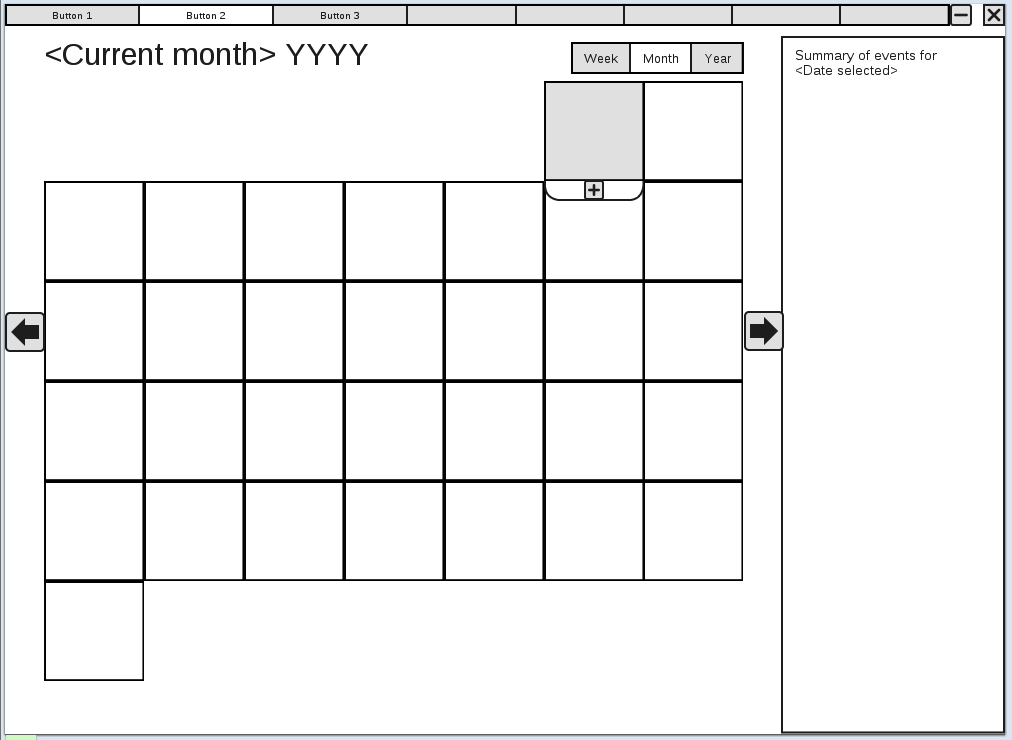
\includegraphics[scale=0.5,angle=90]{CMCLGDRMonth.png}
\caption{Month View}
\label{fig:monthview}
\end{figure}

\begin{figure}[hb]
\centering
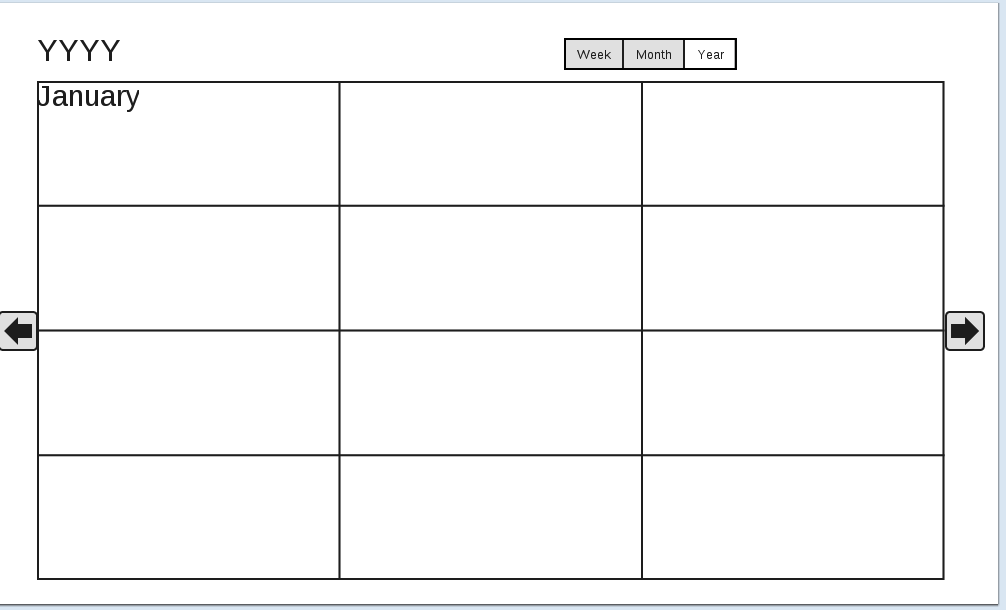
\includegraphics[scale=0.5,angle=90]{CMCLGDRYear.png}
\caption{Year View}
\label{fig:yearview}
\end{figure}

\end{document}

%%%%%%%%%%%%%%%%%%%%%%%%%%%%%%%%%%%%%%%%%%%%%%%%%%%%%%%%%%%%%%%%%%%%%%%
